\title{2021 年高考数学 天津卷}
\date{}
\maketitle

\section*{一、选择题}
在每小题给出的四个选项中，只有一项是符合题目要求的．

\begin{question}[points=5]
设集合 $A = \{-1,0,1\}$，$B = \{1,3,5\}$，$C = \{0,2,4\}$，则 $(A \cap B) \cup C =$（   ）
\begin{choices}
  \item $\{0\}$
  \item $\{0,1,3,5\}$
  \item $\{0,1,2,4\}$
  \item $\{0,2,3,4\}$
\end{choices}
\begin{solution}
\textbf{答案：}C

\textbf{分析：}根据交集并集的定义即可求出.

\textbf{详解：}$\because A = \{-1,0,1\}$，$B = \{1,3,5\}$，$C = \{0,2,4\}$，$\therefore A \cap B = \{1\}$，$\therefore (A \cap B) \cup C = \{0,1,2,4\}$. 故选：C.
\end{solution}
\end{question}

\begin{question}[points=5]
已知 $a \in \mathbb{R}$，则“$a > 6$”是“$a^2 > 36$”的（   ）
\begin{choices}
  \item 充分不必要条件
  \item 必要不充分条件
  \item 充要条件
  \item 既不允分也不必要条件
\end{choices}
\begin{solution}
\textbf{答案：}A

\textbf{分析：}由充分条件、必要条件的定义判断即可得解.

\textbf{详解：}若 $a > 6$，则 $a^2 > 36$，故充分性成立；若 $a^2 > 36$，则 $a > 6$ 或 $a < -6$，推不出 $a > 6$，故必要性不成立；所以“$a > 6$”是“$a^2 > 36$”的充分不必要条件. 故选：A.
\end{solution}
\end{question}

\begin{question}[points=5]
函数 $y = \frac{\ln |x|}{x^2 + 2}$ 的图像大致为（   ）

\begin{center}
  
\includegraphics[width=.38\linewidth]{question-3-1.jpg}
\end{center}

\begin{center}
  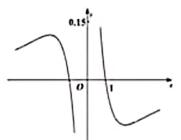
\includegraphics[width=.38\linewidth]{question-3-2.jpg}
\end{center}
\begin{choices}
  \item A
  \item B
  \item C
  \item D
\end{choices}
\begin{solution}
\textbf{答案：}B

\textbf{分析：}由函数为偶函数可排除 AC，再由当 $x \in (0,1)$ 时，$f(x) < 0$，排除 D，即可得解.

\textbf{详解：}设 $y = f(x) = \frac{\ln |x|}{x^2 + 2}$，定义域为 $\{ x | x \neq 0 \}$，关于原点对称，又 $f(-x) = \frac{\ln | -x |}{(-x)^2 + 2} = f(x)$，所以函数为偶函数，排除 AC；当 $x \in (0,1)$ 时，$\ln |x| < 0$，$x^2 + 2 > 0$，所以 $f(x) < 0$，排除 D. 故选：B.
\end{solution}
\end{question}

\begin{question}[points=5]
从某网络平台推荐的影视作品中抽取400部，统计其评分数据，将所得400个评分数据分为8组：$[66,70)$，$[70,74)$，$\ldots$，$[94,98]$，并整理得到如下的频率分布直方图，则评分在区间 $[82,86)$ 内的影视作品数量是（   ）

\begin{center}
  
\includegraphics[width=.38\linewidth]{question-4-1.jpg}
\end{center}
\begin{choices}
  \item 20
  \item 40
  \item 64
  \item 80
\end{choices}
\begin{solution}
\textbf{答案：}D

\textbf{分析：}利用频率分布直方图可计算出评分在区间 $[82,86)$ 内的影视作品数量.

\textbf{详解：}由频率分布直方图可知，评分在区间 $[82,86)$ 内的影视作品数量为 $400 \times 0.05 \times 4 = 80$. 故选：D.
\end{solution}
\end{question}

\begin{question}[points=5]
设 $a = \log_2 0.3$，$b = \log_{\frac{1}{2}} 0.4$，$c = 0.4^{0.3}$，则 $a$，$b$，$c$ 的大小关系为（   ）
\begin{choices}
  \item $a < b < c$
  \item $c < a < b$
  \item $b < c < a$
  \item $a < c < b$
\end{choices}
\begin{solution}
\textbf{答案：}D

\textbf{分析：}根据指数函数和对数函数的性质求出 $a$，$b$，$c$ 的范围即可求解.

\textbf{详解：}$\because \log_2 0.3 < \log_2 1 = 0$，$\therefore a < 0$；$\because \log_{\frac{1}{2}} 0.4 = -\log_2 0.4 = \log_2 \frac{5}{2} > \log_2 2 = 1$，$\therefore b > 1$；$\because 0 < 0.4^{0.3} < 0.4^0 = 1$，$\therefore 0 < c < 1$；$\therefore a < c < b$. 故选：D.
\end{solution}
\end{question}

\begin{question}[points=5]
两个圆锥的底面是一个球的同一截面，顶点均在球面上，若球的体积为 $\frac{32\pi}{3}$，两个圆锥的高之比为 $1:3$，则这两个圆锥的体积之和为（   ）

\begin{center}
  
\includegraphics[width=.38\linewidth]{question-6-1.jpg}
\end{center}
\begin{choices}
  \item $3\pi$
  \item $4\pi$
  \item $9\pi$
  \item $12\pi$
\end{choices}
\begin{solution}
\textbf{答案：}B

\textbf{分析：}作出图形，计算球体的半径，可计算得出两圆锥的高，利用三角形相似计算出圆锥的底面圆半径，再利用锥体体积公式可求得结果.

\textbf{详解：}设球半径为 $R$，则 $\frac{4\pi R^3}{3} = \frac{32\pi}{3}$，得 $R=2$，所以 $AB=4$，设圆锥高之比为 $1:3$，则 $BD=1$，$AD=3$，$CD \perp AB$，由 $\triangle ACD \sim \triangle CBD$，得 $CD = \sqrt{AD \cdot BD} = \sqrt{3}$，所以两个圆锥的体积之和为 $\frac{1}{3}\pi \cdot CD^2 \cdot (AD+BD) = \frac{1}{3}\pi \cdot 3 \cdot 4 = 4\pi$．故选：B.
\end{solution}
\end{question}

\begin{question}[points=5]
若 $2^a = 5^b = 10$，则 $\frac{1}{a} + \frac{1}{b} =$（   ）
\begin{choices}
  \item $-1$
  \item $\lg 7$
  \item $1$
  \item $\log_{7} 10$
\end{choices}
\begin{solution}
\textbf{答案：}C

\textbf{分析：}由已知表示出 $a$，$b$，再由换底公式可求.

\textbf{详解：}$\because 2^a = 5^b = 10$，$\therefore a = \log_2 10$，$b = \log_5 10$，$\therefore \frac{1}{a} + \frac{1}{b} = \frac{1}{\log_2 10} + \frac{1}{\log_5 10} = \lg 2 + \lg 5 = \lg 10 = 1$．故选：C.
\end{solution}
\end{question}

\begin{question}[points=5]
已知双曲线 $\frac{x^2}{a^2} - \frac{y^2}{b^2} = 1$ ($a > 0$, $b > 0$) 的右焦点与抛物线 $y^2 = 2px$ ($p > 0$) 的焦点重合，抛物线的准线交双曲线于 $A$，$B$ 两点，交双曲线的渐近线于 $C$，$D$ 两点，若 $|CD| = 2|AB|$，则双曲线的离心率为（   ）
\begin{choices}
  \item $\sqrt{2}$
  \item $\sqrt{3}$
  \item $2$
  \item $3$
\end{choices}
\begin{solution}
\textbf{答案：}A

\textbf{分析：}设公共焦点为 $(c,0)$，可得准线为 $x=-c$，代入双曲线及渐近线方程，结合线段长度比值可得 $a^2 = \frac{1}{2}c^2$，再由双曲线离心率公式即可得解.

\textbf{详解：}设双曲线与抛物线的公共焦点为 $(c,0)$，则准线为 $x=-c$，代入双曲线方程得 $y = \pm \frac{b^2}{a}$，所以 $|AB| = \frac{2b^2}{a}$；渐近线方程为 $y = \pm \frac{b}{a}x$，代入 $x=-c$ 得 $y = \pm \frac{bc}{a}$，所以 $|CD| = \frac{2bc}{a}$，由 $|CD| = \sqrt{2}|AB|$ 得 $\frac{2bc}{a} = \sqrt{2} \cdot \frac{2b^2}{a}$，即 $c = \sqrt{2}b$，所以 $a^2 = c^2 - b^2 = 2b^2 - b^2 = b^2$，即 $a=b$，离心率 $e = \frac{c}{a} = \sqrt{2}$．故选：A.
\end{solution}
\end{question}

\begin{question}[points=5]
设 $a \in \mathbb{R}$，函数 $f(x) = \begin{cases} \cos(2\pi x - 2\pi a), & x < a \\ x^2 - 2(a+1)x + a^2 + 5, & x \ge a \end{cases}$，若 $f(x)$ 在区间 $(0, +\infty)$ 内恰有6个零点，则 $a$ 的取值范围是（   ）
\begin{choices}
  \item $\left(2, \frac{9}{4}\right] \cup \left(\frac{5}{2}, \frac{11}{4}\right]$
  \item $\left(\frac{7}{4}, 2\right) \cup \left(\frac{5}{2}, \frac{11}{4}\right)$
  \item $\left(2, \frac{9}{4}\right] \cup \left[\frac{11}{4}, 3\right)$
  \item $\left(\frac{7}{4}, 2\right) \cup \left[\frac{11}{4}, 3\right)$
\end{choices}
\begin{solution}
\textbf{答案：}A

\textbf{分析：}由 $x^2 - 2(a+1)x + a^2 + 5 = 0$ 最多有2个根，可得 $\cos(2\pi x - 2\pi a)=0$ 至少有4个根，分别讨论当 $x < a$ 和 $x \ge a$ 时两个函数零点个数情况，再结合考虑即可得出.

\textbf{详解：}略
\end{solution}
\end{question}

\section*{二、填空题}
本大题共6小题，每小题5分，共30分，试题中包含两个空的，答对1个的给3分，全部答对的给5分．

\begin{question}[points=5]
$i$ 是虚数单位，复数 $\frac{9+2i}{2+i} =$ .
\fillin[{$4-i$}]
\begin{solution}
\textbf{答案：}$4-i$

\textbf{分析：}利用复数的除法化简可得结果.

\textbf{详解：}$\frac{9+2i}{2+i} = \frac{(9+2i)(2-i)}{(2+i)(2-i)} = \frac{20-5i}{5} = 4-i$.
\end{solution}
\end{question}

\begin{question}[points=5]
在 $\left(2x^3 + \frac{1}{x}\right)^6$ 的展开式中，$x^6$ 的系数是.
\fillin[{$160$}]
\begin{solution}
\textbf{答案：}$160$

\textbf{分析：}求出二项式的展开式通项，令 $x$ 的指数为6即可求出.

\textbf{详解：}$T_{r+1} = C_6^r (2x^3)^{6-r} \left(\frac{1}{x}\right)^r = 2^{6-r} C_6^r x^{18-4r}$，令 $18-4r=6$，得 $r=3$，所以系数为 $2^3 C_6^3 = 160$.
\end{solution}
\end{question}

\begin{question}[points=5]
若斜率为 $\sqrt{3}$ 的直线与 $y$ 轴交于点 $A$，与圆 $x^2 + (y-1)^2 = 1$ 相切于点 $B$，则 $|AB| =$ .
\fillin[{$\sqrt{3}$}]
\begin{solution}
\textbf{答案：}$\sqrt{3}$

\textbf{分析：}设直线 $AB$ 的方程为 $y = \sqrt{3}x + b$，则点 $A(0,b)$，利用直线 $AB$ 与圆相切求出 $b$ 的值，求出 $AC$，利用勾股定理可求得 $|AB|$.

\textbf{详解：}设直线 $AB$ 的方程为 $y = \sqrt{3}x + b$，则 $A(0,b)$，圆圆心 $C(0,1)$，半径 $1$，由 $\frac{|b-1|}{\sqrt{(\sqrt{3})^2+1}} = 1$，得 $|b-1|=2$，解得 $b=-1$ 或 $b=3$，则 $|AC|=2$，又 $|BC|=1$，所以 $|AB| = \sqrt{2^2-1^2} = \sqrt{3}$.
\end{solution}
\end{question}

\begin{question}[points=5]
若 $a > 0$，$b > 0$，则 $\frac{1}{a} + \frac{a}{b^2} + b$ 的最小值为.
\fillin[{$2\sqrt{2}$}]
\begin{solution}
\textbf{答案：}$2\sqrt{2}$

\textbf{分析：}两次利用基本不等式即可求出.

\textbf{详解：}$\because a>0, b>0$，$\therefore \frac{1}{a} + \frac{a}{b^2} + b \ge 2\sqrt{\frac{1}{a} \cdot \frac{a}{b^2}} + b = \frac{2}{b} + b \ge 2\sqrt{\frac{2}{b} \cdot b} = 2\sqrt{2}$，当且仅当 $\frac{1}{a} = \frac{a}{b^2}$ 且 $\frac{2}{b} = b$，即 $a=b=\sqrt{2}$ 时取等，所以最小值为 $2\sqrt{2}$.
\end{solution}
\end{question}

\begin{question}[points=5]
甲、乙两人在每次猜谜活动中各猜一个谜语，若一方猜对且另一方猜错，则猜对的一方获胜，否则本次平局，已知每次活动中，甲、乙猜对的概率分别为 $\frac{5}{6}$ 和 $\frac{1}{5}$，且每次活动中甲、乙猜对与否互不影响，各次活动也互不影响，则一次活动中，甲获胜的概率为，3次活动中，甲至少获胜2次的概率为.
\fillin[{$\frac{2}{3}$；$\frac{20}{27}$}]
\begin{solution}
\textbf{答案：}$\frac{2}{3}$；$\frac{20}{27}$

\textbf{分析：}根据甲猜对乙没有才对可求出一次活动中，甲获胜的概率；在3次活动中，甲至少获胜2次分为甲获胜2次和3次都获胜求解.

\textbf{详解：}一次活动中，甲获胜的概率为 $\frac{5}{6} \times \left(1-\frac{1}{5}\right) = \frac{5}{6} \times \frac{4}{5} = \frac{2}{3}$；3次活动中，甲至少获胜2次的概率为 $C_3^2 \left(\frac{2}{3}\right)^2 \times \frac{1}{3} + \left(\frac{2}{3}\right)^3 = \frac{12}{27} + \frac{8}{27} = \frac{20}{27}$.
\end{solution}
\end{question}

\begin{question}[points=5]
在边长为1的等边三角形 $ABC$ 中，$D$ 为线段 $BC$ 上的动点，$DE \perp AB$ 且交 $AB$ 于点 $E$，$DF // AB$ 且交 $AC$ 于点 $F$，则 $|2\overrightarrow{BE} + \overrightarrow{DF}|$ 的值为；$(\overrightarrow{DE} + \overrightarrow{DF}) \cdot \overrightarrow{DA}$ 的最小值为.
\fillin[{$1$；$\frac{11}{20}$}]
\begin{solution}
\textbf{答案：}$1$；$\frac{11}{20}$

\textbf{分析：}设 $BE = x$，由 $(2\overrightarrow{BE} + \overrightarrow{DF})^2$ 可求出；将 $(\overrightarrow{DE} + \overrightarrow{DF}) \cdot \overrightarrow{DA}$ 化为关于 $x$ 的关系式即可求出最值.

\textbf{详解：}设 $BE = x$，$x \in (0, \frac{1}{2})$，则 $BD=2x$，$DE=\sqrt{3}x$，$DC=1-2x$，$\triangle DFC$ 为等边三角形，边长为 $1-2x$，$DE \perp DF$，则 $(2\overrightarrow{BE} + \overrightarrow{DF})^2 = 4x^2 + 4x(1-2x)\cos 0^\circ + (1-2x)^2 = 1$，所以 $|2\overrightarrow{BE} + \overrightarrow{DF}|=1$；$(\overrightarrow{DE}+\overrightarrow{DF})\cdot\overrightarrow{DA} = (\overrightarrow{DE}+\overrightarrow{DF})\cdot(\overrightarrow{DE}+\overrightarrow{EA}) = \overrightarrow{DE}^2 + \overrightarrow{DF}\cdot\overrightarrow{EA} = (\sqrt{3}x)^2 + (1-2x)(1-x) = 5x^2 -3x+1 = 5\left(x-\frac{3}{10}\right)^2 + \frac{11}{20}$，所以当 $x=\frac{3}{10}$ 时，最小值为 $\frac{11}{20}$.
\end{solution}
\end{question}

\section*{三、解答题}
本大题共5小题，共75分，解答应写出文字说明，证明过程或演算步骤．

\begin{question}[points=14]
在 $\triangle ABC$，角 $A, B, C$ 所对的边分别为 $a, b, c$，已知 $\sin A : \sin B : \sin C = 2 : 1 : \sqrt{2}$，$b = \sqrt{2}$．

（I）求 $a$ 的值；

（II）求 $\cos C$ 的值；

（III）求 $\sin\left(2C - \frac{\pi}{6}\right)$ 的值．
\begin{solution}
\textbf{答案：}$a=2\sqrt{2}$；$\cos C = \frac{3}{4}$；$\frac{3\sqrt{21}-1}{16}$

\textbf{分析：}（I）由正弦定理可得 $a:b:c = 2:1:\sqrt{2}$，即可求出；
（II）由余弦定理即可计算；
（III）利用二倍角公式求出 $2C$ 的正弦值和余弦值，再由两角差的正弦公式即可求出.

\textbf{详解：}（I）由正弦定理得 $a:b:c = 2:1:\sqrt{2}$，$\because b = \sqrt{2}$，$\therefore a = 2\sqrt{2}$，$c=2$；
（II）$\cos C = \frac{a^2+b^2-c^2}{2ab} = \frac{8+2-4}{2\times 2\sqrt{2}\times \sqrt{2}} = \frac{6}{8} = \frac{3}{4}$；
（III）$\because \cos C = \frac{3}{4}$，$\therefore \sin C = \frac{\sqrt{7}}{4}$，$\sin 2C = 2\sin C \cos C = \frac{3\sqrt{7}}{8}$，$\cos 2C = 2\cos^2 C -1 = \frac{9}{8}-1 = \frac{1}{8}$，$\sin\left(2C - \frac{\pi}{6}\right) = \sin 2C \cos \frac{\pi}{6} - \cos 2C \sin \frac{\pi}{6} = \frac{3\sqrt{7}}{8} \times \frac{\sqrt{3}}{2} - \frac{1}{8} \times \frac{1}{2} = \frac{3\sqrt{21} - 1}{16}$.
\end{solution}
\end{question}

\begin{question}[points=15]
如图，在棱长为2的正方体 $ABCD - A_1B_1C_1D_1$ 中，$E$ 为棱 $BC$ 的中点，$F$ 为棱 $CD$ 的中点．

（I）求证：$D_1F //$ 平面 $A_1EC_1$；

（II）求直线 $AC_1$ 与平面 $A_1EC_1$ 所成角的正弦值；

（III）求二面角 $A - A_1C_1 - E$ 的正弦值．

\begin{center}
  
\includegraphics[width=.38\linewidth]{question-17-1.jpg}
\end{center}
\begin{solution}
\textbf{答案：}（I）证明见解析；（II）$\frac{\sqrt{3}}{9}$；（III）$\frac{1}{3}$

\textbf{分析：}（I）建立空间直角坐标系，求出 $\overrightarrow{D_1F}$ 及平面 $A_1EC_1$ 的一个法向量 $\vec{m}$，证明 $\overrightarrow{D_1F} \perp \vec{m}$，即可得证；
（II）求出 $\overrightarrow{AC_1}$，由 $\sin\theta = |\cos\langle\vec{m},\overrightarrow{AC_1}\rangle|$ 运算即可得解；
（III）求得平面 $AA_1C_1$ 的一个法向量 $\overrightarrow{DB}$，由 $\cos\langle\overrightarrow{DB},\vec{m}\rangle = \frac{\overrightarrow{DB}\cdot\vec{m}}{|\overrightarrow{DB}||\vec{m}|}$ 结合同角三角函数的平方关系即可得解.

\textbf{详解：}（I）以 $A$ 为原点，$AB, AD, AA_1$ 分别为 $x, y, z$ 轴建立空间直角坐标系，则 $A(0,0,0)$，$A_1(0,0,2)$，$B(2,0,0)$，$C(2,2,0)$，$D(0,2,0)$，$C_1(2,2,2)$，$D_1(0,2,2)$，$E(2,1,0)$，$F(1,2,0)$，$\overrightarrow{D_1F} = (1,0,-2)$，$\overrightarrow{A_1C_1} = (2,2,0)$，$\overrightarrow{A_1E} = (2,1,-2)$，设平面 $A_1EC_1$ 的法向量 $\vec{m} = (x_1,y_1,z_1)$，则 $\begin{cases} \vec{m}\cdot\overrightarrow{A_1C_1}=2x_1+2y_1=0 \\ \vec{m}\cdot\overrightarrow{A_1E}=2x_1+y_1-2z_1=0 \end{cases}$，取 $x_1=2$，得 $\vec{m}=(2,-2,1)$，$\because \overrightarrow{D_1F}\cdot\vec{m}=2-2=0$，$\therefore \overrightarrow{D_1F} \perp \vec{m}$，又 $D_1F \not\subset$ 平面 $A_1EC_1$，$\therefore D_1F //$ 平面 $A_1EC_1$；
（II）$\overrightarrow{AC_1} = (2,2,2)$，设直线 $AC_1$ 与平面 $A_1EC_1$ 所成角为 $\theta$，则 $\sin\theta = |\cos\langle\vec{m},\overrightarrow{AC_1}\rangle| = \frac{|\vec{m}\cdot\overrightarrow{AC_1}|}{|\vec{m}||\overrightarrow{AC_1}|} = \frac{|2\times2+(-2)\times2+1\times2|}{\sqrt{2^2+(-2)^2+1^2}\sqrt{2^2+2^2+2^2}} = \frac{2}{3\times 2\sqrt{3}} = \frac{\sqrt{3}}{9}$；
（III）平面 $AA_1C_1$ 的一个法向量为 $\overrightarrow{DB} = (2,-2,0)$，$\cos\langle\overrightarrow{DB},\vec{m}\rangle = \frac{\overrightarrow{DB}\cdot\vec{m}}{|\overrightarrow{DB}||\vec{m}|} = \frac{2\times2+(-2)\times(-2)+0\times1}{\sqrt{4+4}\sqrt{4+4+1}} = \frac{8}{2\sqrt{2}\times3} = \frac{2\sqrt{2}}{3}$，则二面角 $A-A_1C_1-E$ 的正弦值为 $\sqrt{1-\left(\frac{2\sqrt{2}}{3}\right)^2} = \frac{1}{3}$.
\end{solution}
\end{question}

\begin{question}[points=15]
已知椭圆 $\frac{x^2}{a^2} + \frac{y^2}{b^2} = 1$ ($a > b > 0$) 的右焦点为 $F$，上顶点为 $B$，离心率为 $\frac{2\sqrt{5}}{5}$，且 $|BF| = \sqrt{5}$．

（I）求椭圆的方程；

（II）直线 $l$ 与椭圆有唯一的公共点 $M$，与 $y$ 轴的正半轴交于点 $N$，过 $N$ 与 $BF$ 垂直的直线交 $x$ 轴于点 $P$．若 $MP // BF$，求直线 $l$ 的方程．
\begin{solution}
\textbf{答案：}（I）$\frac{x^2}{5} + y^2 = 1$；（II）$x - y + \sqrt{6} = 0$

\textbf{分析：}（I）求出 $a$ 的值，结合 $c$ 的值可得出 $b$ 的值，进而可得出椭圆的方程；
（II）设点 $M(x_0,y_0)$，分析出直线 $l$ 的方程为 $\frac{x_0 x}{5} + y_0 y = 1$，求出点 $P$ 的坐标，根据 $MP // BF$ 可得出 $k_{MP} = k_{BF}$，求出 $x_0$、$y_0$ 的值，即可得出直线 $l$ 的方程.

\textbf{详解：}（I）$F(c,0)$，$B(0,b)$，$|BF| = \sqrt{c^2+b^2} = a = \sqrt{5}$，离心率 $e = \frac{c}{a} = \frac{2\sqrt{5}}{5}$，得 $c=2$，$b = \sqrt{a^2-c^2} = 1$，所以椭圆方程为 $\frac{x^2}{5} + y^2 = 1$；
（II）设 $M(x_0,y_0)$ 为椭圆上一点，则椭圆在 $M$ 处的切线方程为 $\frac{x_0 x}{5} + y_0 y = 1$，令 $x=0$ 得 $N\left(0,\frac{1}{y_0}\right)$，$BF$ 斜率为 $k_{BF} = -\frac{b}{c} = -\frac{1}{2}$，则 $PN$ 方程为 $y = 2x + \frac{1}{y_0}$，令 $y=0$ 得 $P\left(-\frac{1}{2y_0},0\right)$，$k_{MP} = \frac{y_0}{x_0+\frac{1}{2y_0}} = \frac{2y_0^2}{2x_0 y_0+1}$，由 $MP // BF$ 得 $\frac{2y_0^2}{2x_0 y_0+1} = -\frac{1}{2}$，整理得 $(x_0+5y_0)^2=0$，所以 $x_0 = -5y_0$，代入椭圆方程得 $\frac{25y_0^2}{5}+y_0^2=6y_0^2=1$，$y_0 = \frac{\sqrt{6}}{6}$，$x_0 = -\frac{5\sqrt{6}}{6}$，所以直线 $l$ 方程为 $\frac{-\frac{5\sqrt{6}}{6}x}{5} + \frac{\sqrt{6}}{6}y = 1$，即 $x - y + \sqrt{6}=0$.
\end{solution}
\end{question}

\begin{question}[points=15]
已知 $\{a_n\}$ 是公差为 $2$ 的等差数列，其前 $8$ 项和为 $64$．$\{b_n\}$ 是公比大于 $0$ 的等比数列，$b_1 = 4$，$b_3 - b_2 = 48$．

（I）求 $\{a_n\}$ 和 $\{b_n\}$ 的通项公式；

（II）记 $c_n = b_{2n} + \frac{1}{b_n}$，$n \in \mathbb{N}^*$．

（i）证明 $\{c_n^2 - c_{2n}\}$ 是等比数列；

（ii）证明 $\sum_{k=1}^n \frac{a_k a_{k+1}}{c_k^2 - c_{2k}} < 2\sqrt{2}$（$n \in \mathbb{N}^*$）．
\begin{solution}
\textbf{答案：}（I）$a_n = 2n-1$，$b_n = 4^n$；（II）证明见解析

\textbf{分析：}（I）由等差数列的求和公式运算可得 $\{a_n\}$ 的通项，由等比数列的通项公式运算可得 $\{b_n\}$ 的通项公式；
（II）（i）运算可得 $c_n^2 - c_{2n} = 2 \cdot 4^n$，结合等比数列的定义即可得证；
（ii）放缩得 $\frac{a_n a_{n+1}}{c_n^2 - c_{2n}} < \frac{4n^2}{2 \cdot 2^{2n}} = \frac{1}{2} \cdot \frac{n}{2^{n-1}}$，进而可得 $\sum_{k=1}^n \frac{a_k a_{k+1}}{c_k^2 - c_{2k}} < \frac{1}{2} \sum_{k=1}^n \frac{k}{2^{k-1}}$，结合错位相减法即可得证.

\textbf{详解：}（I）$\{a_n\}$ 公差 $d=2$，前8项和 $S_8 = 8a_1 + \frac{8\times7}{2}\times2 = 64$，得 $a_1=1$，$a_n = 2n-1$；$\{b_n\}$ 公比 $q>0$，$b_1=4$，$b_3-b_2=4q^2-4q=48$，解得 $q=4$（负舍），$b_n=4^n$；
（II）（i）$c_n = 4^{2n} + \frac{1}{4^n}$，$c_n^2 - c_{2n} = \left(4^{2n} + \frac{1}{4^n}\right)^2 - \left(4^{4n} + \frac{1}{4^{2n}}\right) = 2\cdot4^n$，$\because c_n^2 - c_{2n} \neq 0$，且 $\frac{c_{n+1}^2 - c_{2(n+1)}}{c_n^2 - c_{2n}} = \frac{2\cdot4^{n+1}}{2\cdot4^n} = 4$，$\therefore \{c_n^2 - c_{2n}\}$ 是等比数列；
（ii）$a_k a_{k+1} = (2k-1)(2k+1) = 4k^2-1 < 4k^2$，$c_k^2 - c_{2k} = 2\cdot4^k = 2\cdot2^{2k}$，$\therefore \frac{a_k a_{k+1}}{c_k^2 - c_{2k}} < \frac{4k^2}{2\cdot2^{2k}} = \frac{1}{2}\cdot\frac{k}{2^{k-1}}$，$\sum_{k=1}^n \frac{a_k a_{k+1}}{c_k^2 - c_{2k}} < \frac{1}{2} \sum_{k=1}^n \frac{k}{2^{k-1}}$，令 $T_n = \sum_{k=1}^n \frac{k}{2^{k-1}}$，则 $\frac{1}{2}T_n = \sum_{k=1}^n \frac{k}{2^k}$，两式相减得 $\frac{1}{2}T_n = 1+\frac{1}{2}+\frac{1}{2^2}+\cdots+\frac{1}{2^{n-1}} - \frac{n}{2^n} = 2\left(1-\frac{1}{2^n}\right) - \frac{n}{2^n} = 2 - \frac{n+2}{2^n}$，$T_n = 4 - \frac{n+2}{2^{n-1}}$，$\therefore \sum_{k=1}^n \frac{a_k a_{k+1}}{c_k^2 - c_{2k}} < \frac{1}{2}\left(4 - \frac{n+2}{2^{n-1}}\right) = 2 - \frac{n+2}{2^n} < 2\sqrt{2}$．
\end{solution}
\end{question}

\begin{question}[points=16]
已知 $a > 0$，函数 $f(x) = ax - xe^x$．

（I）求曲线 $y = f(x)$ 在点 $(0, f(0))$ 处的切线方程；

（II）证明 $f(x)$ 存在唯一的极值点；

（III）若存在 $a$，使得 $f(x) \le a + b$ 对任意 $x \in \mathbb{R}$ 成立，求实数 $b$ 的取值范围．
\begin{solution}
\textbf{答案：}（I）$y = (a-1)x$；（II）证明见解析；（III）$[-e, +\infty)$

\textbf{分析：}（I）求出 $f(x)$ 在 $x=0$ 处的导数，即切线斜率，求出 $f(0)$，即可求出切线方程；
（II）令 $f'(x)=0$，可得 $a = (x+1)e^x$，则可化为证明 $y=a$ 与 $y=g(x)$ 仅有一个交点，利用导数求出 $g(x)$ 的变化情况，数形结合即可求解；
（III）令 $h(x) = (x^2 - x - 1)e^x$，$x > -1$，题目等价于存在 $x \in (-1, +\infty)$，使得 $h(x) \le b$，即 $b \ge h(x)_{\min}$，利用导数即可求出 $h(x)$ 的最小值.

\textbf{详解：}（I）$f'(x) = a - (x+1)e^x$，$f'(0) = a-1$，$f(0)=0$，切线方程为 $y = (a-1)x$；
（II）令 $f'(x)=0$ 得 $a = (x+1)e^x$，令 $g(x) = (x+1)e^x$，$g'(x) = (x+2)e^x$，当 $x \in (-\infty, -2)$ 时 $g'(x)<0$，$g(x)$ 递减；当 $x \in (-2, +\infty)$ 时 $g'(x)>0$，$g(x)$ 递增，$x \to -\infty$ 时 $g(x) \to 0^-$，$g(-1)=0$，$x \to +\infty$ 时 $g(x) \to +\infty$，故 $y=a$ 与 $y=g(x)$ 仅有一个交点，设交点为 $(m, a)$，则 $m > -1$，且 $f'(m)=0$，当 $x < m$ 时 $f'(x)>0$，$f(x)$ 递增；当 $x > m$ 时 $f'(x)<0$，$f(x)$ 递减，所以 $x=m$ 为极大值点，故 $f(x)$ 存在唯一的极值点；
（III）由（II）知 $f(x)_{\max} = f(m)$，且 $a = (m+1)e^m$，$m>-1$，则 $f(m)-a = (m^2 - m -1)e^m$，令 $h(x) = (x^2 - x - 1)e^x$，$x>-1$，则 $h'(x) = (x^2 + x -2)e^x = (x-1)(x+2)e^x$，当 $x \in (-1,1)$ 时 $h'(x)<0$，$h(x)$ 递减；当 $x \in (1, +\infty)$ 时 $h'(x)>0$，$h(x)$ 递增，$h(x)_{\min} = h(1) = -e$，存在 $a$ 使 $f(x) \le a+b$ 对任意 $x$ 成立等价于存在 $x>-1$ 使 $h(x) \le b$，即 $b \ge h(x)_{\min} = -e$，所以 $b$ 的取值范围是 $[-e, +\infty)$.
\end{solution}
\end{question}

